\chapter{FUNDAMENTAÇÃO TEÓRICO-METODOLÓGICA}


O primeiro passo na expressão de um gene é a transcrição. No processo de transcrição muitos fatores internos ou externos, na célula, podem influenciar induzindo ou reprimindo a expressão dos diversos genes codificados no genoma do organismo. Fatores externos desafiantes, como estresses bióticos e abióticos, até mecanismos moleculares intrínsecos podem desencadear, direta ou indiretamente, a ativação da expressão gênica espaço-temporal.

%achar definições em livros para complementar inserir uma figura para explicar visualmente
A transcrição consiste na formação do RNA a partir do DNA, para que a transcrição ocorra é necessário a ação de uma enzima chamada RNA-polimerase, essa enzima se conecta na sequência de DNA, próximo a região onde está o local de inicio da transcrição (LIT) e se move sobre o DNA, no sentido contrario ao LIT formando o RNA, a transcrição é iniciada exatamente após o LIT. Por sua vez para que a RNA-polimerase consiga se conectar no DNA é imprescindível a ação conjunta de proteínas especiais que se conectam a determinados segmentos de DNA.

% pesquisar sobre fatores de transcrição basicos para a transcrição
Essas proteínas são chamadas de fatores de transcrição (TFs), elas podem se conectar distante da RNA-polimerase ou próximo a RNA-polimerase formando um complexo de vários fatores de transcrição juntamente com a RNA-polimerase. Os segmentos de DNA em que os TFs se ligam são pequenos(5 a 20 nucleotídeos), e são chamados de elementos regulatórios. Geralmente os elementos regulatórios estão  localizados em uma região antes do local de inicio da transcrição, como mostrado na figura 1. Esta região recebe o nome de região promotora, ela será responsável de promover um gene, para ser expresso. A ligação dos TFs nos elementos regulatórios interfere no posicionamento correto da RNA-polimerase, na separação das fitas de DNA para permitir o inicio da transcrição, e na liberação da RNA-polimerase quando a transcrição se inicia e consequentemente na transcrição de um gene. Quando ocorre a transcrição parte do RNA transcrito ira formar posteriormente proteínas, que são essenciais para a sobrevivência do organismo, estas proteínas podem até mesmo ser TFs que irão ativar outros genes.

A transcrição esta diretamente ligada a respostas das células a estímulos, como mudanças hormonais internamente em um organismo, ou externamente como estresses abióticos e bióticos. Os estresses abióticos são causados por fatores não vivos como a alteração de temperatura e mudança climática. Os estresses bióticos são causados por organismos vivos como bactérias, vírus, parasitas e insetos.


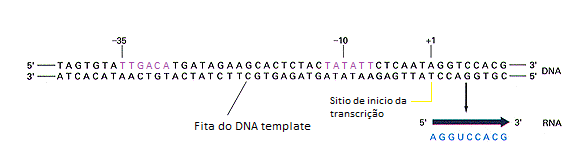
\includegraphics[]{imagens/regiaopromotora}

Figura 1. Região promotora, com dois elementos regulatórios.


No amplo conjunto de fatores de transcrição, existem aqueles que quando ligados nos elementos regulatórios irão ativar as respostas da célula a estresses abióticos. Em organismos vegetais os estresses abióticos que mais prejudicam são: a seca, alta salinização e baixas temperaturas. Esses fatores de transcrição quando ligados aos elementos regulatórios irão desencadear uma série de eventos que resultara na proteção da célula e sua tolerância a estresses. Na \textit{Arabdopsis}, uma planta modelo amplamente utilizada em pesquisas de genética molecular nas plantas, os fatores de transcrição relacionados a estresses abióticos são agrupados em classes (ou famílias), uma das principais classes é a Dehydration Responsive Element Binding Proteins (DREB), que por sua vez pertence a família Ethylene Responsive Element (ERF), uma importante família de fatores de transcrição de respostas a estresses. O DREB é subdividido em duas subclasses: DREB1/CBF e DREB2 que são induzidas pelo frio e desidratação, respectivamente \cite{Agarwal2006}.

Segundo Agarwal et al.\cite{Agarwal2006} estresses abióticos e bióticos influenciam negativamente na sobrevivência e na larga produção de grãos. Culturas como soja, arroz e trigo que são amplamente usadas na alimentação mundial são prejudicadas pelos estresses que muitas vezes impedem uma alta produtividade. O entendimento dos DREBs na regulação de um gene é de grande importância para o desenvolvimento de plantas tolerantes a estresses.


Existem vários métodos computacionais desenvolvidos para encontrar elementos regulatórios nos genes de diversos organismos, Das e Dai \cite{Das2007} classificou os métodos existentes em três grupos:
\begin{itemize}
\item Os baseados em sequências promotoras de genes que são regulados pelos mesmos fatores de transcrição (genes co-regulados), estes métodos se concentram em apenas um único genoma.

\item Os que utilizam sequencias promotoras ortólogas, que são sequencias de DNA similares a várias espécies, indicando que estas espécies derivaram de um ancestral comum, também chamados de métodos de rastros filogenéticos.

\item Os métodos que combinam rastros filogenéticos e sequencias promotoras de genes co-regulados.
\end{itemize}


Os métodos baseados em genes co-regulados ainda podem ser divididos em dois subgrupos: de predição baseada em palavras e predição probabilística.

%%%%
%Fazer uma tabela listando os principais algoritmos dos três grupos
%%%%
Algoritmos de predição baseada em palavras computam todas as possíveis subsequências que podem ocorrer, através de diferentes sequências promotoras. Encontrado o número de frequência de uma subsequência, este deve ser comparado com o número de frequência esperada. Depois, são utilizados métodos estatísticos para avaliar a significância da sequência observada \cite{Rombauts2003}.

Os modelos de predição probabilística, geralmente utilizam matriz de peso e os parâmetros do modelo são estimado usando o princípio de inferência bayesiana. Há varias implementações baseadas no método probabilístico, entre estas técnicas destacam as técnicas estatísticas como \textit{EM} método e \textit{Gibb sampling}, técnicas de aprendizado de máquina e técnicas de \textit{Ensemble} \cite{Das2007}.

Os algoritmos baseados em rastros filogenéticos assumem que elementos regulatórios são regiões conservadas no DNA e não sofreram muitas mutações ao longo da evolução. Esses algoritmos comparam sequências promotoras de genes ortólogos de múltiplas espécies para identificar os elementos regulatórios.

Por último os algoritmos que combinam as técnicas probabilísticas e de rastros filogenéticos, que integram dois importantes aspectos dos elementos regulatórios, a sobre-representação e a conservação dos elementos regulatórios entre múltiplas espécies \cite{Das2007}. Algumas das implementações dos modelos citados estão listadas na tabela 2.1.

Dos modelos apresentados, a predição baseada em palavras mostrou-se eficiente na busca de elementos regulatórios em organismos eucarióticos mas problemática em organismos procarióticos, devido ao tamanho dos elementos regulatórios nos eucarióticos serem menores do que nos procarióticos. A predição baseada em rastros filogenéticos, mostrou-se muito eficiente em organismos procarióticos, mas é necessário as sequencias de varias espécies, para fazer as comparações, com o avanço do sequenciamento do genoma das espécies este método ficara cada vez mais expressivo. O modelo de predição probabilística também tem-se mostrado eficiente na busca de elementos regulatórios em grandes genomas, uma das técnicas que se destaca com  grande eficiência na busca de elementos regulatórios dentro dos modelos que utilizam aprendizado de máquina é a de \textit{support vector machine} (SVM).

Até o presente momento poucos foram os trabalhos que se dedicaram exclusivamente na busca DREBs nas plantas. Recentemente Wang et al. \cite{Wang2009} criou um método utilizando SVM para encontrar genes que eram expressos quando expostos a fatores abióticos na \textit{Arabidopsis}. Eles utilizaram sequencias de DNA de regiões promotoras de genes da \textit{Arabidopsis}, que possuía elementos regulatórios que se conectavam a DREBs como dados positivos e sequencias aleatórias da região promotora representando os dados negativos, primeiramente foi aplicado o algoritmo HexDiff \cite{Chan2005} para análise dos hexâmeros sobre-representados nas sequencias e então as sequencias promotoras dos genes foram classificadas com o SVM, discriminando os as sequencias de genes que eram alvos de DREBs das que não eram.


\begin{table}[h!]
\begin{center}
  \begin{tabular}{| l | c | }
    \hline
    Algoritmos     & Referências       \\ \hline \hline

    \multicolumn{2}{|c|}{Algoritmos de predição baseada em palavras}  \\ \hline

    Oligo-Analysis & \cite{Helden1998} \\ \hline
    YMF            & \cite{Sinha2003}  \\ \hline
    MITRA          & \cite{Eskin2002}  \\ \hline

    \multicolumn{2}{|c|}{Algoritmos de predição probabilística}       \\ \hline

    MEME           & \cite{Bailey2006}   \\ \hline
    Gibbs sampling & \cite{Lawrence1993} \\ \hline
    AlignACE       & \cite{Roth1998}     \\ \hline
    Motif Sampler  & \cite{Thijs2002}    \\ \hline

    \multicolumn{2}{|c|}{Algoritmos baseados em rastros filogenéticos} \\ \hline

    Footprinter    & \cite{Blanchette2002} \\ \hline
    PHYLONET       & \cite{Wang2005}       \\ \hline
    PhyloScan      & \cite{Carmack2007}    \\ \hline

    \multicolumn{2}{|c|}{Algoritmos baseados em rastros filogenéticos e predição probabilística}             \\ \hline

    OrthoMEME      & \cite{Carmack2007}  \\ \hline
    PhyloCon       & \cite{Wang2003}     \\ \hline
    PhyME          & \cite{Sinha2004}    \\ \hline

    \hline

  \end{tabular}
\end{center}
  \caption{Implementações de modelos de predição}
\end{table}


Atualmente existem poucas ferramentas dedicadas à descoberta de elementos regulatórios em plantas, a maior parte das soluções são baseadas em fungos, mamíferos e insetos como a Drosophila. Das ferramentas dedicadas a plantas a maior parte é baseada na planta modelo Arabidopsis.